% !TEX program = pdflatex
% =============================================================================
% Final-project presentation (English --- the version for the actual demo).
% COMPILES WITH pdflatex.  No external theme, no fontspec, no extra fonts:
% everything is built from beamer's default + manual styling, so it builds on
% any vanilla TeX Live / MiKTeX install on Windows without metropolis/Fira.
% Build:  pdflatex presentation.tex   (run twice for the page-total counter).
%
% Video frames use placeholder TikZ "thumbnails"; replace each
%   \thumb{<label>}
% with  \includegraphics[width=\linewidth,height=4.2cm,keepaspectratio]{<file>}
% once you have a screenshot frame from each mp4.
% =============================================================================
\documentclass[aspectratio=169,10pt]{beamer}

% ---------- Robust, dependency-free academic styling ----------
\usepackage[T1]{fontenc}
\usepackage{lmodern}
\usepackage{amsmath, amssymb}
\usepackage{booktabs}
\usepackage{array}
\usepackage{tikz}
\usetikzlibrary{positioning, arrows.meta, fit, shapes.geometric, calc}
\usepackage{xcolor}
\usepackage{graphicx}

\setbeamertemplate{navigation symbols}{}
\setbeamersize{text margin left=9mm, text margin right=9mm}

% palette
\definecolor{accent}{HTML}{2A6DB0}
\definecolor{accent2}{HTML}{C0392B}
\definecolor{accent3}{HTML}{1B7A5A}
\definecolor{soft}{HTML}{EEF2F7}
\definecolor{ink}{HTML}{222222}
\definecolor{muted}{HTML}{6B7280}

\setbeamercolor{frametitle}{fg=white, bg=accent}
\setbeamercolor{title}{fg=accent}
\setbeamercolor{author}{fg=ink}
\setbeamercolor{institute}{fg=muted}
\setbeamercolor{structure}{fg=accent}
\setbeamercolor{alerted text}{fg=accent2}
\setbeamercolor{itemize item}{fg=accent}
\setbeamercolor{itemize subitem}{fg=accent}
\setbeamercolor{block title}{fg=white, bg=accent}
\setbeamercolor{block body}{bg=soft, fg=ink}
\setbeamerfont{frametitle}{series=\bfseries}
\setbeamerfont{title}{series=\bfseries, size=\LARGE}
\setbeamerfont{block title}{series=\bfseries, size=\small}

% full-width coloured title bar
\setbeamertemplate{frametitle}{%
  \nointerlineskip%
  \begin{beamercolorbox}[wd=\paperwidth, ht=3.0ex, dp=1.3ex, leftskip=9mm, rightskip=9mm]{frametitle}%
    \usebeamerfont{frametitle}\insertframetitle%
  \end{beamercolorbox}%
}
% clean footline: short title left, frame N / total right
\setbeamertemplate{footline}{%
  \hbox{\begin{beamercolorbox}[wd=\paperwidth, ht=2.4ex, dp=1.0ex, leftskip=9mm, rightskip=9mm]{}%
    {\tiny\color{muted}\insertshorttitle}\hfill{\tiny\color{muted}\insertframenumber\,/\,\inserttotalframenumber}%
  \end{beamercolorbox}}%
}

% a small "video thumbnail" placeholder (swap for \includegraphics later)
\newcommand{\thumb}[1]{%
  \begin{tikzpicture}
    \node[draw=accent!50, fill=soft, rounded corners=2pt,
          minimum width=4.7cm, minimum height=3.3cm,
          text width=4.3cm, align=center, font=\footnotesize] {%
      {\bfseries\color{accent}[\,video\,]}\\[3pt]%
      \color{ink} #1\\[4pt]%
      {\tiny\color{muted}replace with a frame}};
  \end{tikzpicture}%
}

\title[Stereo-VLM Manipulation]{Stereo-Vision Closed-Loop Manipulation\\with Open-Vocabulary Grounding}
\author{Yingjun Lan \quad Jinhao Zhang \quad Zhengxiang Liu}
\institute{School of Artificial Intelligence, Shanghai Jiao Tong University}
\date{Final Project Presentation}

\begin{document}

% ===================== TITLE =====================
\begin{frame}[plain]
\titlepage
\end{frame}

% ===================== MOTIVATION =====================
\begin{frame}{The language$\,\to\,$action gap}
\begin{columns}[T,onlytextwidth]
\column{0.56\textwidth}
\textbf{Goal.} From a free-form instruction to robot joint torques.
\vspace{4pt}
\begin{itemize}
    \item Instruction lives in a \alert{semantic} space.
    \item Control lives in a \alert{metric} space.
    \item End-to-end VLAs (RT-2) learn the map directly\dots
    \item \dots but need \alert{large teleoperated datasets} and generalize poorly out of distribution.
\end{itemize}
\column{0.40\textwidth}
\centering
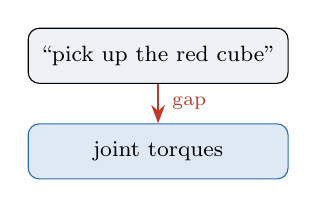
\begin{tikzpicture}[font=\footnotesize]
\node[draw, rounded corners, fill=soft, minimum width=3.3cm, minimum height=0.7cm] (n) {``pick up the red cube''};
\node[draw, rounded corners, fill=accent!15, draw=accent, minimum width=3.3cm, minimum height=0.7cm, below=0.5cm of n] (a) {joint torques};
\draw[->, >=Stealth, thick, accent2] (n) -- node[right, font=\scriptsize] {\,gap} (a);
\end{tikzpicture}
\end{columns}
\end{frame}

% ===================== CORE IDEA =====================
\begin{frame}{Core idea: decompose, don't learn end-to-end}
Route a \alert{frozen} VLM through geometry and a symbolic planner.
\vspace{8pt}
\begin{columns}[T,onlytextwidth]
\column{0.52\textwidth}
\textbf{Instead of one big learned map:}
\begin{itemize}
    \item \textbf{Perception} --- OWLv2 grounds the named object.
    \item \textbf{Geometry} --- stereo triangulation $\to$ metric 3D.
    \item \textbf{Planning} --- VLM emits a 7-primitive DSL.
    \item \textbf{Control} --- OSC executor runs it.
\end{itemize}
\column{0.46\textwidth}
\textbf{Why this matters for a small team:}
\begin{itemize}
    \item \alert{Training-free} --- no teleoperation data.
    \item Inspectable: each stage is auditable.
    \item Runs on a single T4 GPU.
\end{itemize}
\end{columns}
\end{frame}

% ===================== EMPHASIS 1: VLA WORKFLOW =====================
\begin{frame}{Workflow --- closed-loop cycle}
\centering
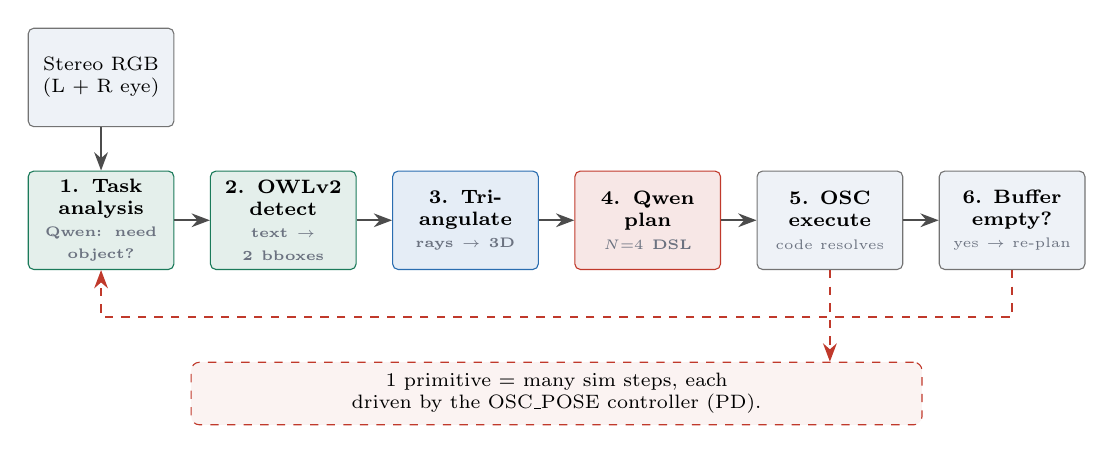
\begin{tikzpicture}[font=\scriptsize,
  box/.style={rectangle, draw=black!55, rounded corners=2pt, fill=soft, minimum width=1.85cm, minimum height=1.25cm, align=center, inner sep=2pt, text width=1.70cm},
  det/.style={rectangle, draw=accent3, fill=accent3!12, rounded corners=2pt, minimum width=1.85cm, minimum height=1.25cm, align=center, inner sep=2pt, text width=1.70cm, font=\scriptsize\bfseries},
  geo/.style={rectangle, draw=accent, fill=accent!12, rounded corners=2pt, minimum width=1.85cm, minimum height=1.25cm, align=center, inner sep=2pt, text width=1.70cm, font=\scriptsize\bfseries},
  vlm/.style={rectangle, draw=accent2, fill=accent2!12, rounded corners=2pt, minimum width=1.85cm, minimum height=1.25cm, align=center, inner sep=2pt, text width=1.70cm, font=\scriptsize\bfseries},
  arr/.style={->, >=Stealth, thick, black!70}]
\node[det] (d1) {\textbf{1. Task analysis}\\\textcolor{muted}{\tiny Qwen: need object?}};
\node[det, right=0.45cm of d1] (d2) {\textbf{2. OWLv2 detect}\\\textcolor{muted}{\tiny text $\to$ 2 bboxes}};
\node[geo, right=0.45cm of d2] (d3) {\textbf{3. Triangulate}\\\textcolor{muted}{\tiny rays $\to$ 3D}};
\node[vlm, right=0.45cm of d3] (d4) {\textbf{4. Qwen plan}\\\textcolor{muted}{\tiny $N{=}4$ DSL}};
\node[box, right=0.45cm of d4] (d5) {\textbf{5. OSC execute}\\\textcolor{muted}{\tiny code resolves}};
\node[box, right=0.45cm of d5] (d6) {\textbf{6. Buffer empty?}\\\textcolor{muted}{\tiny yes $\to$ re-plan}};
\node[box, above=0.55cm of d1] (img) {Stereo RGB\\(L + R eye)};
\draw[arr] (img) -- (d1);
\draw[arr] (d1) -- (d2);
\draw[arr] (d2) -- (d3);
\draw[arr] (d3) -- (d4);
\draw[arr] (d4) -- (d5);
\draw[arr] (d5) -- (d6);
\draw[arr, dashed, accent2] (d6.south) -- ++(0,-0.6) -| (d1.south);
% --- zoom into the "execute" node (5): 1 primitive = many sim steps ---
\node[draw=accent2, dashed, rounded corners=3pt, fill=accent2!6, text width=9cm, align=center, font=\scriptsize, inner sep=4pt] (zoom) at ($(d1)!0.5!(d6)+(0,-2.2)$) {%
\alert{1 primitive = many sim steps}, each driven by the OSC\_POSE controller (PD).};
\draw[arr, dashed, accent2] (d5.south) -- (d5.south |- zoom.north);
\end{tikzpicture}
\vspace{4pt}

\end{frame}

% ===================== OWLv2 =====================
\begin{frame}{Open-vocabulary grounding with OWLv2}
\textbf{Problem.} Asking the VLM to regress boxes is unreliable for small objects.
\begin{itemize}
    \item Ground the target with \alert{OWLv2} (\texttt{owlv2-base-patch16-ensemble}, $\sim$0.6B).
    \item Query text comes from the instruction (target noun) or a per-trial override.
    \item Runs \alert{once per round on both eyes} with the same query.
    \item Returns highest-scoring box $[x_1,y_1,x_2,y_2]$ per eye; threshold $0.05$.
    \item Round fails only if \emph{both} eyes miss; single-eye miss still triangulates.
\end{itemize}
\vspace{3pt}
\footnotesize\textit{Decoupling:} the VLM understands \emph{what} to grasp; OWLv2 finds \emph{where}; geometry recovers \emph{how far}.
\end{frame}

% ===================== STEREO + TRIANGULATION =====================
\begin{frame}{Binocular stereo \& ray triangulation}
\textbf{Setup.} Inject \texttt{left\_eye} / \texttt{right\_eye} into MuJoCo, $0.50$\,m baseline, look-at table center.

Back-project each box center to a viewing ray:
\[
\mathbf{d}_c = R_c\big[(u{-}c_x)/f_x,\;(v{-}c_y)/f_y,\;-1\big]^{\!\top},\quad
\mathbf{r}_c(t)=\mathbf{o}_c+t\,\hat{\mathbf{d}}_c
\]
Closest point of two rays (least squares):
\[
(t^\star,s^\star)=\arg\min_{t,s}\,\big\|\mathbf{o}_L+t\hat{\mathbf{d}}_L-\mathbf{o}_R-s\hat{\mathbf{d}}_R\big\|^2,\quad
\mathbf{p}=\tfrac{1}{2}\big(\mathbf{r}_L(t^\star)+\mathbf{r}_R(s^\star)\big)
\]
\vspace{-4pt}
\begin{itemize}
    \item Residual gap $>5$\,cm $\Rightarrow$ reject \& re-query (free consistency check).
    \item Generalizes to objects \emph{off} the reference plane (e.g.\ inside a bin), no table-height assumption.
\end{itemize}
\end{frame}

% ===================== DSL =====================
\begin{frame}{RMDL: a seven-primitive motion DSL}
\centering
\footnotesize
\begin{tabular}{@{}lll@{}}
\toprule
\textbf{Primitive} & \textbf{Parameters} & \textbf{Target resolution} \\
\midrule
\texttt{move\_to} & target \{object, above\_object\}, height? & code: \texttt{object\_3d} ($\pm$ height) \\
\texttt{move\_by} & offset $[dx,dy,dz]$, speed & code: $\mathbf{p}_{ee}+$ offset \\
\texttt{descend}  & --- & code: vertical to table contact (plateau) \\
\texttt{rotate}   & rotation $[r,p,y]\!\in\![-1,1]$, speed & code: relative EE orientation \\
\texttt{grasp}    & --- & close gripper (sticky) \\
\texttt{release}  & --- & open gripper (guarded: only over bin) \\
\texttt{wait}     & --- & no-op (fixed duration) \\
\bottomrule
\end{tabular}
\vspace{6pt}
\end{frame}

% ===================== EMPHASIS 2: LM OUTPUT =====================
\begin{frame}{What the language model outputs}
The VLM returns \alert{one JSON object}: a natural-language \texttt{reasoning} trace + an \texttt{actions} list of exactly $N{=}4$ DSL primitives.
\vspace{3pt}

\begin{columns}[T,onlytextwidth]
\column{0.56\textwidth}
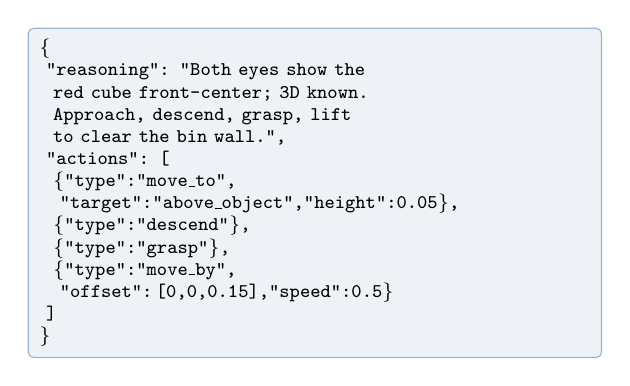
\begin{tikzpicture}
\node[draw=accent!50, fill=soft, rounded corners=2pt, text width=7.0cm, inner sep=4pt, font=\ttfamily\scriptsize, align=left]
{\{\\
\ "reasoning": "Both eyes show the\\
\ \ red cube front-center; 3D known.\\
\ \ Approach, descend, grasp, lift\\
\ \ to clear the bin wall.",\\
\ "actions": [\\
\ \ \{"type":"move\_to",\\
\ \ \ "target":"above\_object","height":0.05\},\\
\ \ \{"type":"descend"\},\\
\ \ \{"type":"grasp"\},\\
\ \ \{"type":"move\_by",\\
\ \ \ "offset":\,[0,0,0.15],"speed":0.5\}\\
\ ]\\
\}};
\end{tikzpicture}

\column{0.42\textwidth}
\footnotesize
\textbf{Why this works:}
\begin{itemize}
    \item \alert{Validated}: malformed JSON / empty array / \texttt{error} field $\to$ retry with a targeted hint (up to 10$\times$).
    \item \alert{No arithmetic}: \texttt{target} is a \emph{keyword} (\texttt{object}), not a coordinate --- code supplies XYZ.
    \item \alert{Strategy, not control}: the VLM chooses \emph{which} primitive; the executor chooses \emph{how far}.
    \item \alert{Deterministic grounding}: OWLv2 (not the VLM) finds the box, so the plan is anchored to a real pixel.
\end{itemize}
\end{columns}
\end{frame}

% ===================== EXECUTION DEPTH =====================
\begin{frame}{Execution: many steps per cycle}
\textbf{One cycle} = the VLM plans $N{=}4$ primitives $\to$ execute them $\to$ re-plan. Each primitive runs as many \alert{sim steps} as needed (until within 5\,mm of its target or it plateaus), so a cycle is dozens of steps.
\vspace{6pt}

\textbf{Execution uses OSC, not a model.} Every step is driven by Robosuite's \alert{OSC\_POSE} controller (PD); Qwen3-VL and OWLv2 run \emph{only} at the start of a cycle.
\vspace{6pt}

\textbf{Inside one sim step} (\alert{no neural net}): read EE pose $\to$ OSC action $\Delta=\text{speed}\cdot(\text{target}{-}\text{ee})$ $+$ sticky gripper $\to$ \texttt{env.step} $\to$ check success.
\vspace{6pt}

\textbf{History snapshots.} After each primitive finishes, a stereo (L$+$R) frame is saved (up to 2); at re-plan the VLM sees the current views \emph{plus} these snapshots.
\end{frame}

% ===================== EMPHASIS 3: VIEWPOINT STUDY =====================
% ===================== VIEWPOINT + BUG (merged) =====================
\begin{frame}{Viewpoints study and result}
\textbf{Viewpoint study.} We tried single-view, dual-view, and binocular stereo. Dual-view already beats single-view, and \alert{binocular stereo is the most practical one} --- so we adopt it.
\vspace{4pt}

\vspace{6pt}

\begin{block}{Result}
Binocular stereo reaches \alert{\textbf{83\%}} over \alert{100} trials.
\end{block}
\end{frame}

% ===================== EMPHASIS 4: DEMO VIDEOS =====================
\begin{frame}{Demonstrations}
\vspace{6pt}
\begin{itemize}
    \item \href{run:./red_cube.mp4}{\textbf{Pick \& place: red cube $\to$ wooden bin}} \\
          \textcolor{muted}{\footnotesize grasp the cube, lift over the bin wall, drop inside, release.}
    \item \href{run:./different_color.mp4}{\textbf{Color transfer: red / green / blue cubes}} \\
          \textcolor{muted}{\footnotesize the same OWLv2 + stereo + VLM pipeline handles all colours without retraining.}
    \item \href{run:./failed.mp4}{\textbf{Failure case: rotating grasp of bottle \& milk}} \\
          \textcolor{muted}{\footnotesize the gripper rotates to align with non-cylindrical objects --- shape or occlusion causes failure.}
\end{itemize}
\vspace{6pt}
\end{frame}

% ===================== DANCE DEMO =====================
\begin{frame}{Demonstration - Free-motion ``dance''}
\centering
\includegraphics[width=0.85\linewidth,height=0.75\textheight,keepaspectratio]{../dance_thumb.png}
\end{frame}

% ===================== EMPHASIS 5: RL TRAINING =====================
\begin{frame}{RL branch: GRPO-style LoRA fine-tuning of the planner}
\textbf{The planner \emph{is} the policy.} Rather than a separate action head, Qwen3-VL-4B itself is the policy: it emits DSL plans (\texttt{move\_to}/\texttt{descend}/\texttt{grasp}/\texttt{move\_by}/\texttt{release}) that the same \texttt{VLMController} executes with OWLv2 + stereo + the closed loop.
\vspace{4pt}

\begin{columns}[T,onlytextwidth]
\column{0.52\textwidth}
\textbf{Method}
\begin{itemize}
    \item \alert{Only LoRA} of Qwen is trained ($r{=}16,\alpha{=}32$, all-linear); the base model stays 4-bit frozen.
    \item \alert{GRPO-style}: each update fixes the scene seed, samples \texttt{grpo\_group\_size=4} candidate plans, executes each, and updates with the group-relative advantage.
    \item \alert{Reward = task success} (binary $1/0$) on pick-and-place.
\end{itemize}
\column{0.46\textwidth}
\textbf{Config \& status}
\begin{itemize}
    \item Small sample $+$ binary reward $\Rightarrow$ high variance; logprob is recomputed post-hoc (not textbook GRPO).
    \item No ideal final curve yet, and limited by hardware, but the pipeline proved feasible.
    \item Can be used to finish more difficult tasks in future work.
\end{itemize}
\end{columns}
\end{frame}
% ===================== GENERALIZATION (replaces Limitations) =====================
\begin{frame}{Generalization: harder tasks the framework already enables}
The decoupled \emph{what / where / how-far} design plus the re-planning loop make these reachable with \alert{no architectural change} --- only detection targets, prompts, or camera placement change.
\vspace{4pt}
\begin{itemize}
    \item \textbf{Obstacle-aware pick-and-place} \textcolor{accent3}{(easy)} --- add the obstacle as a second OWLv2 target and one prompt rule; the VLM plans a detour before placing.
    \item \textbf{Shape-aware grasp} \textcolor{accent2}{(hard, prompt-only)} --- e.g.\ grasp a cup by its \emph{handle}. The VLM already perceives shape; a grasp-pose prompt lets it choose \emph{where} to grip, while geometry supplies the 3D.
    \item \textbf{Escaping the binocular blind spot} \textcolor{accent}{(camera swap)} --- if OWLv2 misses, let the VLM steer the arm to search; a \emph{wrist-view} camera makes 3D recovery a simple pose-transform of the same ray triangulation.
\end{itemize}
\vspace{4pt}
\footnotesize\textcolor{muted}{Each is a consequence of the same modular stack --- not new learning.}
\end{frame}

% ===================== CONCLUSION =====================
\begin{frame}{Conclusion}
\textbf{Takeaway.} A frozen VLM + open-vocabulary detector + binocular stereo, glued by a 7-primitive DSL and a re-planning loop, performs \alert{training-free} language-guided manipulation.
\vspace{20pt}
\hrule
\vspace{6pt}
\centering\large\textbf{Thank you}
\end{frame}

% ===================== CONTRIBUTIONS =====================
\begin{frame}{References}
\textbf{Selected references}
\begin{itemize}
    \item Mandlekar et al. \emph{Robomimic}, CoRL 2021.
    \item Brohan et al. \emph{RT-2}, CoRL 2023.
    \item Gu et al. \emph{OWLv2} (scaling open-vocabulary detection), CVPR 2024.
    \item Qwen Team. \emph{Qwen3-VL}, 2025.
    \item Zhu et al. \emph{robosuite}, arXiv 2020.
    \item Mittal et al. \emph{Isaac Lab / Isaac Sim}, 2023.
\end{itemize}
\end{frame}

\end{document}
